\documentclass{beamer}
\usepackage[utf8]{inputenc}
\usepackage{default}
\usepackage{listings}
\usepackage{relsize}
\usepackage{graphicx}
\usepackage{multimedia}
\usepackage{soul}
\mode<presentation>{ \usetheme{Singapore} }
\title{ Palestra com nome engraçadinho pra chamar gente }
\subtitle{ A construção do Caos }
\author{ Tomaz Canabrava }

\AtBeginSection[]
{
   \begin{frame}
       \frametitle{Outline}
       \tableofcontents[currentsection]
   \end{frame}
}

\AtBeginSubsection[]
{
   \begin{frame}
       \frametitle{Outline}
       \tableofcontents[currentsection,currentsubsection]
   \end{frame}
}

\begin{document}
\begin{frame} \titlepage \end{frame}

\begin{frame} \frametitle{1940}
    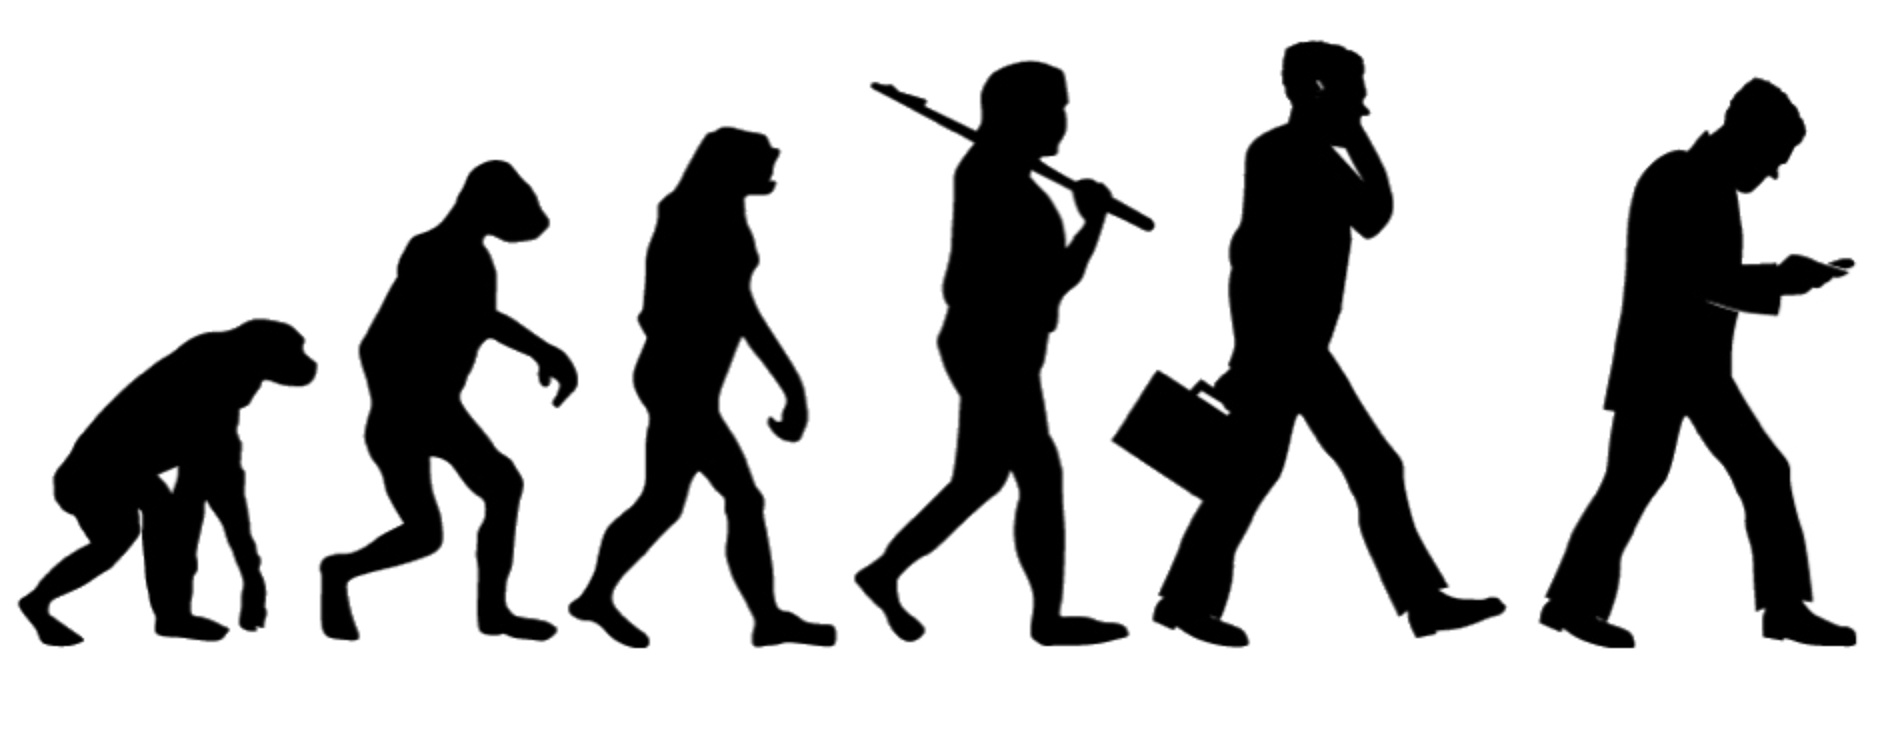
\includegraphics[width=300px]{images/evolution}
\end{frame}

\section { Breve Histórico }
\subsection{ Pré História }
\begin{frame} \frametitle{Invenções Pré-históricas}
    \begin{itemize}
     \item Fogo
     \item Roda
     \item Imprensa
     \pause
     \item Eniac
    \end{itemize}
\end{frame}

\begin{frame} \frametitle{Eniac}
    
\includegraphics[width=300px]{images/eniac}
\end{frame}

\begin{frame} \frametitle{Eniac em 1940}
    \begin{columns}
    \column{0.5\textwidth}
    \begin{itemize}
        \item Base 10
        \pause
        \item 5000 calculos por segundo
        \pause
        \item 5 Milhões pontos de solda manuais
        \pause
        \item 150kw de energia
        \pause
        \item Não cabia no seu bolso.
    \end{itemize}
    \end{columns}
\end{frame}

\begin{frame} \frametitle{Uma olhada em 150kw}
    \begin{itemize}
    \item 3750 lampadas de 40w
    \item Carregar 150 Androids por um Ano
    \item Um Laser Militar (Ainda em Construção)
    \end{itemize}
\end{frame}

\begin{frame} \frametitle{IBM}
    \begin{columns}
        \column{0.5\textwidth}
        ``I think there is a world market for about five computers''

        Thomas J Watson
        \pause
        \column{0.5\textwidth}
        ``Eu acho que existe um mercado mundial para uns cinco computadores''
    \end{columns}
\end{frame}

\begin{frame} \frametitle{1960 e MainFrames}
    \begin{columns}
        \column{0.5\textwidth}
        \begin{itemize}
  \item Transistores
  \item Módulos de Fita
  \item Cartões Perfurados
  \item ``Super computadores''
  \item Terminais burros
  \item Fortran
        \end{itemize}
        \column{0.5\textwidth}
  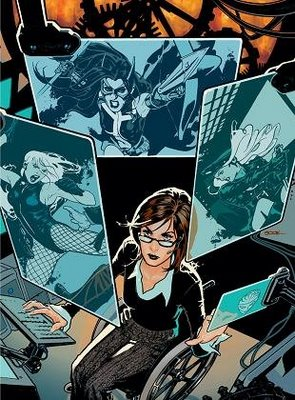
\includegraphics[width=150px]{images/oraculo}
    \end{columns}
\end{frame}
\subsection { Idade das Trevas }
\begin{frame} \frametitle{Fortran}
 \center{“I don't know what the language of the year 2000 will look like, but I know it will be called Fortran.”}
 \linebreak
 \linebreak
 Tony Hoare, ganhador do troféu Turing
 \pause
 \linebreak
 \center{“Não sei como será a linguagem mais usada nos anos 2000, mas sei que ela se chamará fortran.”}
\end{frame}

\begin{frame} \frametitle{Fortran}
    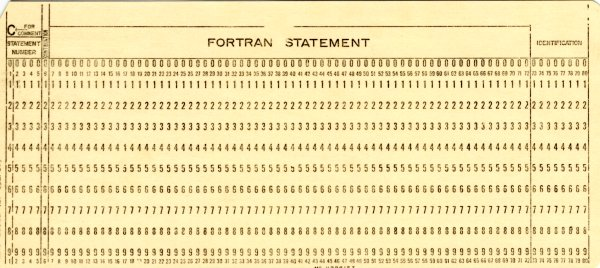
\includegraphics[width=300px]{images/fortran}
\end{frame}

\begin{frame} \frametitle{C e Unix}
    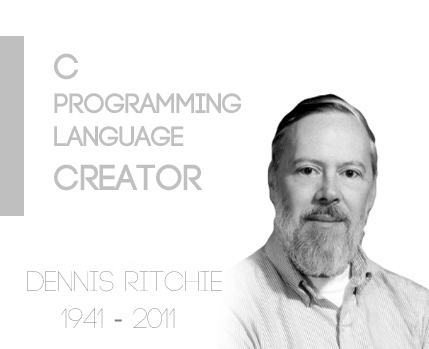
\includegraphics[width=250px]{images/c-unix-creator}
\end{frame}

\begin{frame} \frametitle{ 1980 - 2000, Era dos PC's}
    \begin{itemize}
     \item Menos Potentes
     \item Menos Memória
     \item Menos gastos com Energia
     \item Menos custos de manutenção
     \item ``Pessoais''
     \item 15 diskettes e 99 dolares
    \end{itemize}
\end{frame}

\begin{frame} \frametitle{Windows 3.11}
    \movie[width=300px,height=210px,poster,showcontrols]{}{videos/ballmer-sells-windows.avi}
\end{frame}

\begin{frame}
     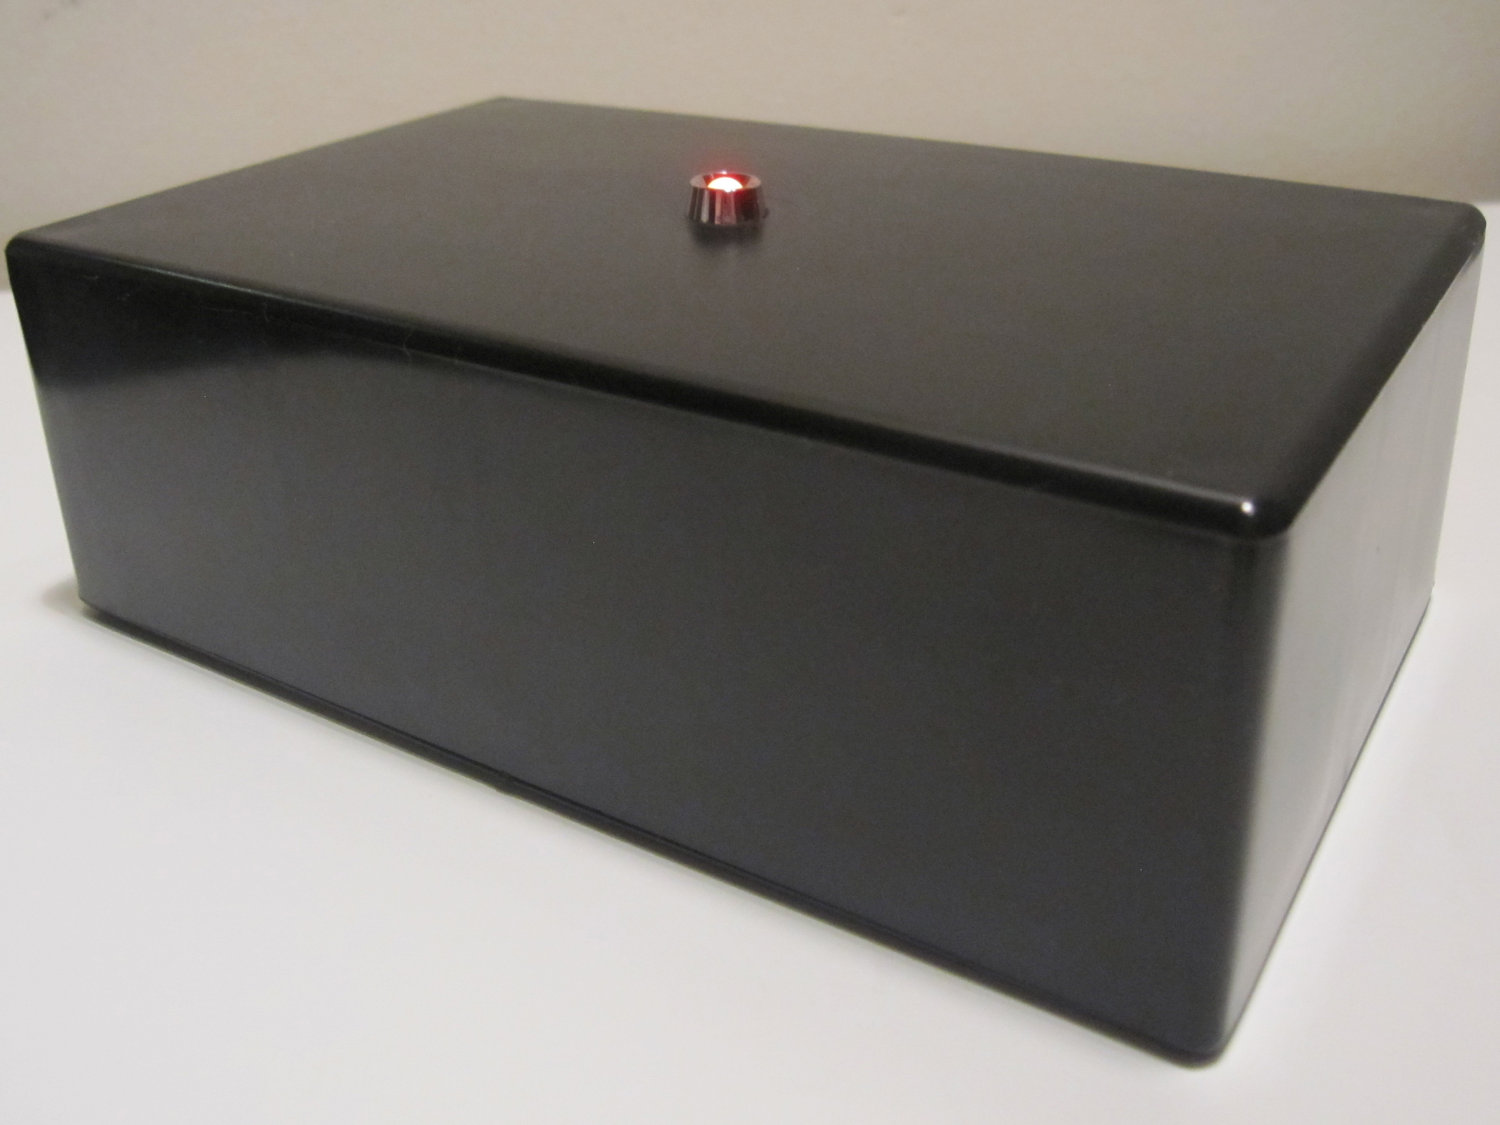
\includegraphics[width=300px]{images/the-internet}
\end{frame}

\subsection{Tempos Modernos}
\begin{frame} \frametitle{A Internet}
     \begin{itemize}
      \item mIRC
      \item icq
      \item netscape
      \item emails
      \item jogos
      \item National Center for Supercomputing Applications
     \end{itemize}
\end{frame}

\begin{frame}
     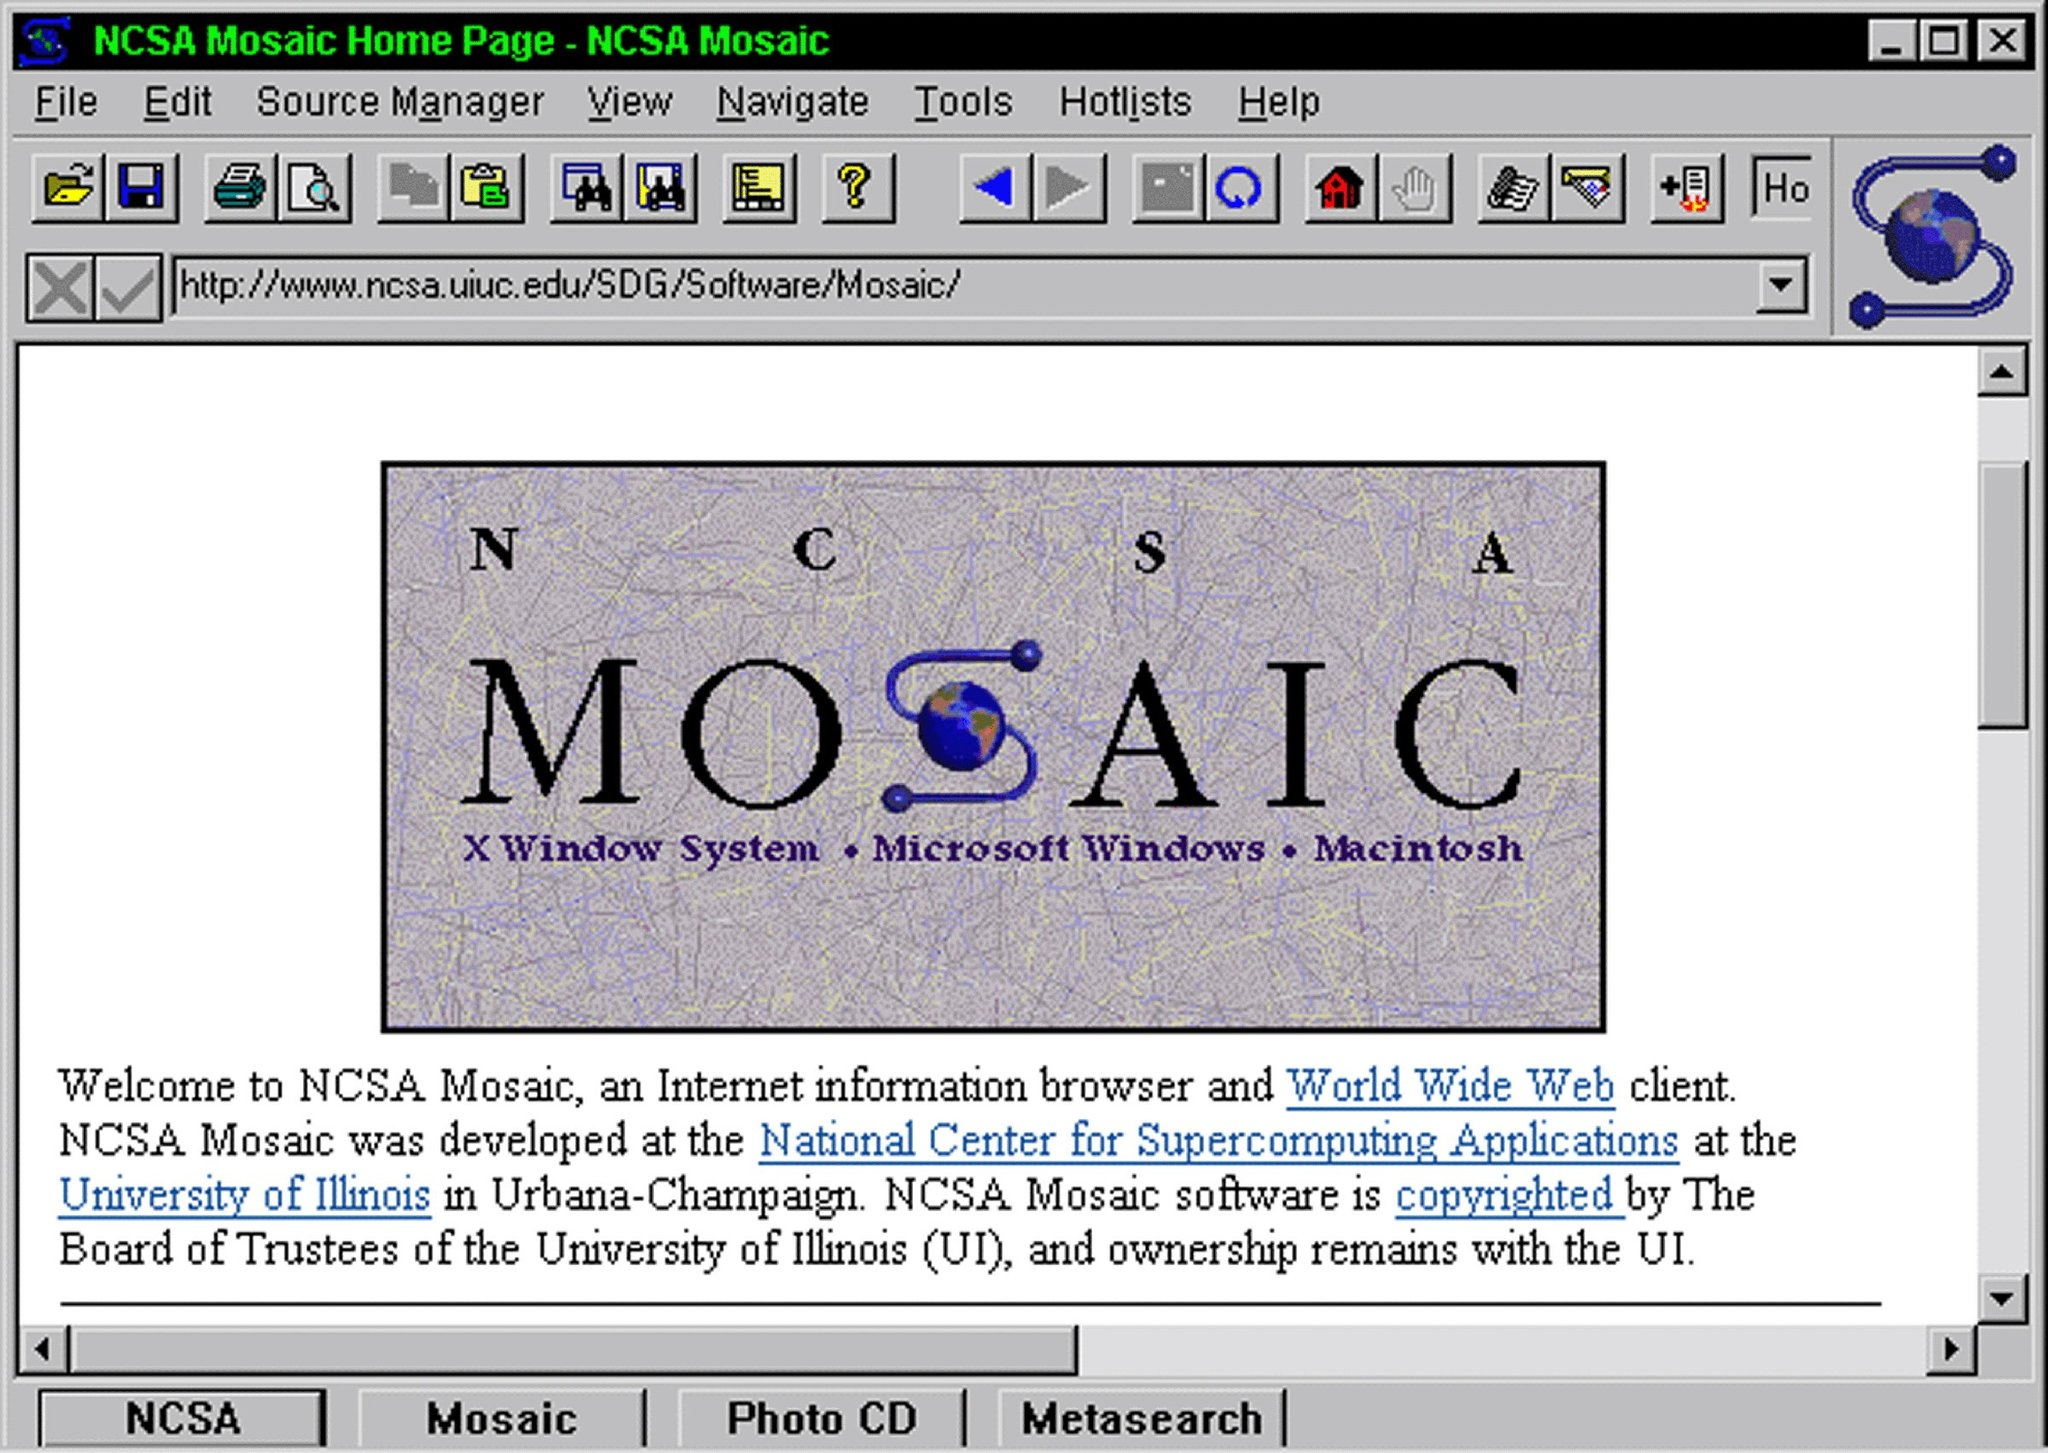
\includegraphics[width=300px]{images/mosaic}
\end{frame}

\begin{frame} \frametitle{Guerra dos Browsers}
    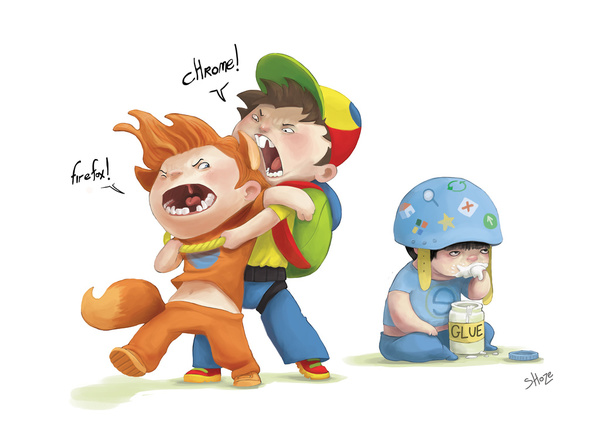
\includegraphics[width=300px]{images/browser-war}
\end{frame}

\begin{frame} \frametitle{Guerra dos Browsers}
    \begin{columns}
        \column{0.5\textwidth}
        \begin{itemize}
  \item Netscape Navigator
  \item Internet Explorer
  \item Opera
  \item Chrome
  \item Firefox
        \end{itemize}
    \end{columns}
\end{frame}

\begin{frame} \frametitle{Guerra dos Browsers}
    \center{O Ganhador? Webkit}
    \begin{itemize}
     \item konqueror
     \item safari
     \item chrome
     \item opera
    \end{itemize}
\end{frame}

\begin{frame}
    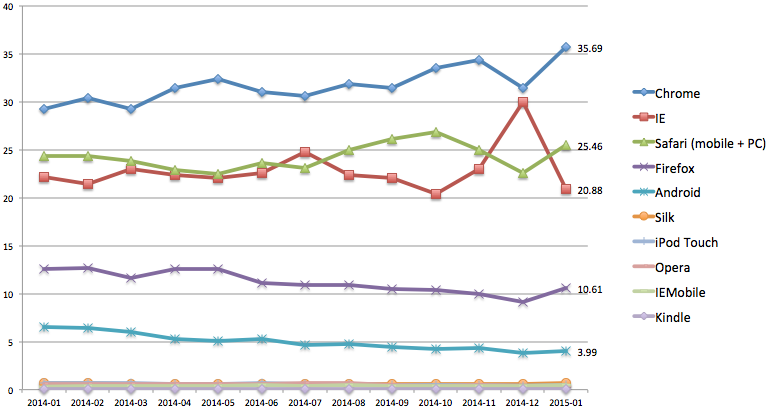
\includegraphics[width=300px]{images/browser-usage}
\end{frame}

\subsection { Tempos Atuais }

\begin{frame} \frametitle{The Cloud e IoT}
    
\includegraphics[width=300px]{images/cloud-striffe}
\end{frame}

\section { É Tanta coisa... }

\subsection{Tudo que temos que lidar}

\begin{frame} \frametitle{Tudo junto e Misturado}
 \begin{itemize}
  \item Computadores
  \item Celulares
  \item Sensores
  \item Dados
  \item Musicas
  \item Carros
  \item Sites
  \item Babás Eletrônicas
 \end{itemize}
\end{frame}

\begin{frame} \frametitle{ E Onde estamos }
    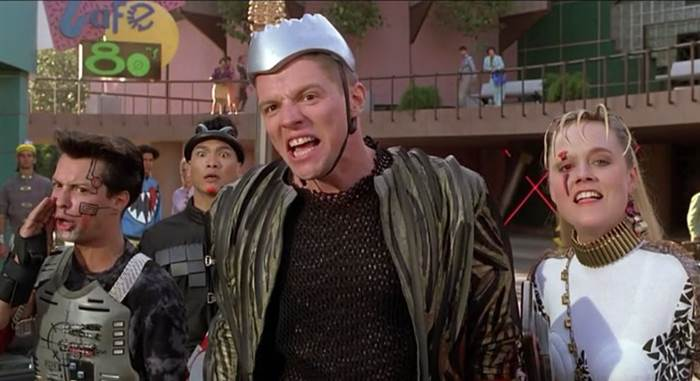
\includegraphics[width=300px]{images/2015}
\end{frame}

\begin{frame} \frametitle{ Celulares }
    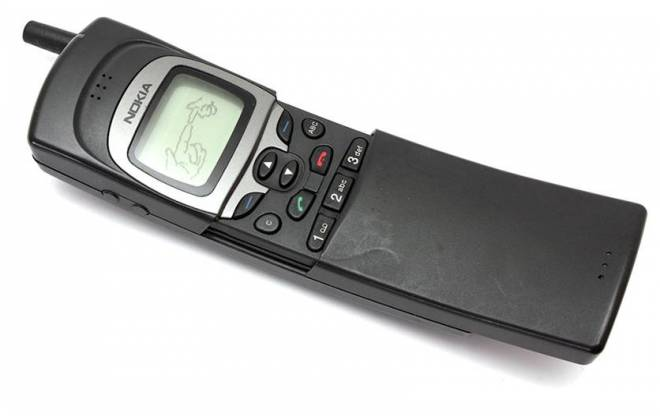
\includegraphics[width=300px]{images/matrix}
\end{frame}

\begin{frame} \frametitle{ Carros }
    \begin{columns}
        \column{0.5\textwidth}
        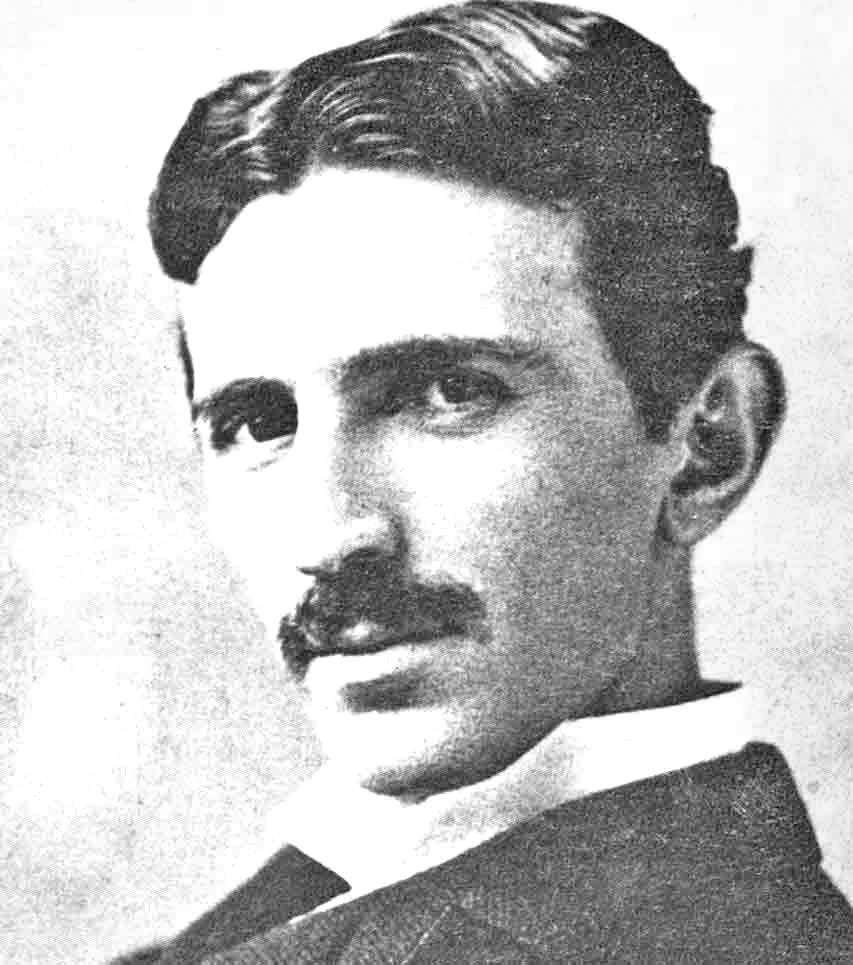
\includegraphics[width=150px]{images/nikola-tesla}
     \end{columns}
\end{frame}

\subsection{Linguagens que temos que trabalhar...}

\begin{frame} \frametitle{Linguagens?}
 \begin{itemize}
  \item C
  \item C++
  \item Csharp
  \item Java
  \item Ruby
  \item Python
  \item JAVA
  \item Javascript
 \end{itemize}
\end{frame}

\begin{frame} \frametitle{ Linguagens Mágicas vs Linguagens Compiladas }
    \framesubtitle { Não existe almoço grátis }
 \begin{center}
\begin{tabular}{ll}
    c & 0.4 mib\\
    c++ & 0.5 mib\\
    fortran & 0.4 mib \\
    java & 40 mib \\
    python & 38 mib \\
    ruby & 45 mib \\
    javascript & 40 mib
 \end{tabular}
 \end{center}
\end{frame}

\begin{frame} \frametitle{ Apressado come ponteiros }
    \framesubtitle { temperados com suor e lágrimas }
 \begin{center}
\begin{tabular}{ll}
    c & 0 ms\\
    c++ & 0.1 ms\\
    fortran & 0 ms \\
    java & 4 ms \\
    python & 20 ms \\
    ruby & 30 ms \\
    javascript & 20 ms
 \end{tabular}
 \end{center}
\end{frame}

\subsection{Tecnologias que temos que trabalhar}
\begin{frame} \frametitle{Troca de Dados?}
    \begin{itemize}
     \item Corba
     \item DBus
     \item XML
     \item JSON
    \end{itemize}
\end{frame}

\begin{frame} \frametitle{Webservices?}
 \begin{itemize}
  \item ssh
  \item HTTP API
  \item FORM REQUESTS
  \item RADATA
 \end{itemize}
\end{frame}

\subsection{Hardwares que vamos usar...}

\begin{frame} \frametitle{Arquiteturas e Hardware?}
    
\includegraphics[width=300px]{images/over--9000}
\end{frame}

\begin{frame} \frametitle{Arquiteturas e Hardware?}

a110x ad8232 adafruitms1438 adafruitss adc121c021 adis16448 adxl335 adxl345
am2315 apds9002 at42qt1070 biss0001 bmpx8x buzzer cjq4435 ds1307 ecs1030
enc03r flex gas gp2y0a grove grovecircularled grovecollision groveehr groveeldriver
groveelectromagnet groveemg grovegsr grovelinefinder groveloudness grovemd
grovemoisture groveo2 grovescam grovespeaker grovevdiv grovewater grovewfs
guvas12d h3lis331dl hcsr04 hm11 hmc5883l hmtrp hp20x ht9170 htu21d hx711 ina132
isd1820 itg3200 joystick12 l298 lcd ldt0028 lol lpd8806 lsm303 m24lr64e max31723
max31855 max44000 max5487 maxds3231m maxsonarez mhz16 mic mlx90614 mma7455 mma7660
mpl3115a2 mpr121 mpu9150 mq303a my9221 nrf24l01 nrf8001 nunchuck otp538u
pca9685 ppd42ns pulsensor rfr359f rgbringcoder rotaryencoder rpr220 servo si114x
sm130 st7735 stepmotor sx6119 ta12200 tcs3414cs th02 tm1637 tsl2561 ttp223 ublox6

\end{frame}

\begin{frame}
 \begin{itemize}
  \item Sensor de Luz
  \item Giroscópio
  \item Sensor de Queda
  \item Sensor de Presença
 \end{itemize}
\end{frame}

\begin{frame} \frametitle{ Restrições de Hardware}
  \begin{center}
\begin{tabular}{ll}
    Memória & 90kb até $ \infty $\\
    Disco & 0b até $ \infty $\\
    Processador & Iniciando em 100mhz
 \end{tabular}
 \end{center}
\end{frame}

\begin{frame} \frametitle{Arquiteturas}
    \begin{itemize}
    \item Tamanho de um char?
    \pause
    \linebreak
    \item 32
    \item 16
    \item 8
    \pause
    \linebreak
    \item \textbf{14}
    \end{itemize}
\end{frame}

\begin{frame}[fragile] \frametitle{Medo no coração dos Fracos}
    \begin{lstlisting}[language=C]

static int field_mask = 0x7 << 10 |
    0xF << 6 | 0xF << 2 | 0x3;

int32_t raw_value = (rx[0] << 24) |
    (rx[1] << 16) | (rx[2] << 8) | rx[3];

raw_value >>= (32 - valid_data);
if (raw_value & (0x1 << valid_data)) {
    raw_value|= ~field_mask;
}

    \end{lstlisting}
\end{frame}

\subsection{Sistemas Operacionais}

\begin{frame} \frametitle{Sistemas Operacionais}
 \begin{itemize}
  \item Familia Windows
  \item Familia Unix
  \item Familia Linux
  \item Sistemas Proprietários
  \item Sistemas Embbed
 \end{itemize}
\end{frame}

\section { Resolvendo o Problema }

\subsection{Linguagens que temos que trabalhar...}
\begin{frame} \frametitle{Linguagens?}
 \begin{itemize}
  \item C
  \item C++
  \item \st{Csharp}
  \item \st{Java}
  \item \st{Ruby}
  \item \st{Python}
  \item \st{JAVA}
  \item \st{Javascript}
 \end{itemize}
\end{frame}

\begin{frame} \frametitle{ Problema do C }
 Imagine controlar Diferentes hardwares

 Ligados ou não na internet

 Ligados ou não em um mesmo periférico

 Em um programa C/C++
\end{frame}

\subsection{IoTivity}

\begin{frame} \frametitle{ IoTivity }
    
\includegraphics[width=300px]{images/iotivity2}
\end{frame}

\begin{frame} \frametitle { IoTivity }
 \textbf{O que é?}
\linebreak
 Framework em C/C++ para trabalhar com internet of things
\linebreak
 \textbf{É de graça?}
\linebreak
 Sim
\linebreak
 \textbf{Devo Usar?}
\linebreak
\pause
 Veja bem...
\end{frame}

\begin{frame} \frametitle{ IoTivity }
    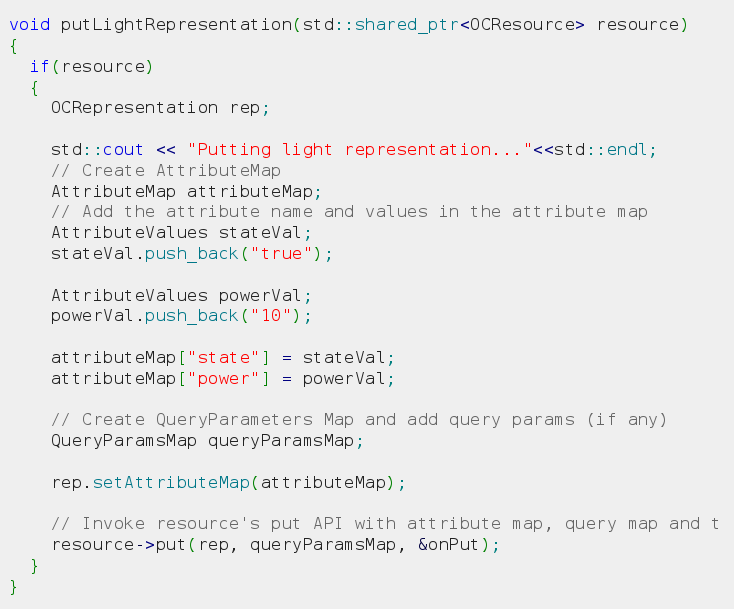
\includegraphics[width=300px]{images/iotivity}
\end{frame}

\begin{frame} \frametitle{ IoTivity }
    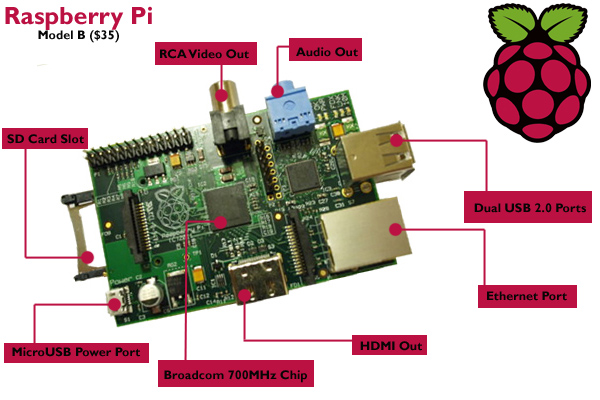
\includegraphics[width=300px]{images/raspy}
\end{frame}

\subsection{Raspaberry Py}
\begin{frame} \frametitle{ Raspaberry - Py }
    \textbf{O que é?}
\linebreak
    Placa e framework para trabalhar com experimentação eletrônica.
\linebreak
    \textbf{É de graça?}
\linebreak
    Não, mas muito barato. (E ótimo presente pra crianças)
\linebreak
    \textbf{Devo Usar?}
\linebreak
    Deve.
\linebreak
    \textbf{Ein?}
    \pause
\linebreak
    Não é tudo que eu não uso que falo mal.
\end{frame}

\begin{frame}[fragile] \frametitle{ Raspaberry - Py}
    \begin{lstlisting}[language=Python]

import time
import picamera
import RPi.GPIO as GPIO

GPIO.setmode(GPIO.BCM)
GPIO.setup(17, GPIO.IN, GPIO.PUD_UP)

with picamera.PiCamera() as camera:
    camera.start_preview()
    GPIO.wait_for_edge(17, GPIO.FALLING)  # new
    camera.capture('/home/pi/Desktop/image.jpg')
    camera.stop_preview()

    \end{lstlisting}
\end{frame}

\subsection{Soletta}

\begin{frame} \frametitle{ Soletta }
        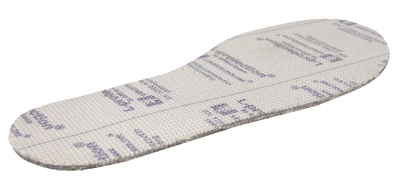
\includegraphics[width=300px]{images/soletta}
\end{frame}

\begin{frame} \frametitle{ Soletta }
    \begin{center}
    Desculpa a falta de logo,

    tá faltando Designers no OpenSource.
    \end{center}
\end{frame}

\begin{frame} \frametitle{ Soletta }
    \textbf{O que é?}
\linebreak
    Um framework em C para trabalhar em auto nivel com devices e IoT
\linebreak
    \textbf{É de graça?}
\linebreak
    Sim, e Open Source.
\linebreak
    \textbf{Devo Usar?}
\linebreak
    Deve.
\linebreak
    \textbf{Código, quero}
\linebreak
    https://github.com/solettaproject/soletta
\end{frame}

\begin{frame}[fragile] \frametitle{ Soletta }
    \begin{lstlisting}
        button(Button) CLICK ->
            PICTURE _(Camera:output="~/image.jpg")
    \end{lstlisting}
    \pause

    Sim, sério.
\end{frame}

\begin{frame} \frametitle{Mas... Mas...}
    
\includegraphics[width=300px]{images/haiku}
\end{frame}

\begin{frame} \frametitle{ Haiku }
    \begin{center}
        Um programador Programa

        Arrastando coisas na tela

        Apenas Ligando os módulos
    \end{center}
\end{frame}
\end{document}
